\chapter{Uncertainty}

\section*{Expected Utility}

In a formal sense, the theory of optimization under uncertainty does not require any new mathematical theory as such. The choice variables lead to random outcomes with objective or subjective probability distributions. The objective functions are appropriate probability weighted averages (expected values). The choices are also subject to some constraints. The general theory developed in the first eight chapters continues to apply. In fact the special structure of problems of choice under uncertainty leads to specific results that were not available in the general mathematics of constrained optimization.

Let us make these ideas a little more precise. Suppose that after the decision at hand has been taken, the world could evolve in any of a number of different ways. These are called different states of the world, or elementary events. Suppose at first that the states are discrete and finite in number, indexed by $i=1,2,\dots,m$. Write $p_i$ for their probabilities, objective or subjective as may be appropriate for the application being considered. These are non-negative and add to one. The economically relevant outcomes in the alternative situations will typically be the levels of income wealth, or profit accruing to the decision-maker. Denote these by $Y_i$. Most of the time I shall take the $Y_i$ to be scalars, but in general they could be vectors. Then we can write a general objective function
\begin{equation*}
F(Y_1, Y_2,\dots, Y_m; p_1, p_2, \dots, p_m)
\end{equation*}
The choice or control variables $x$ will affect some or all of the $Y_i$ and the $p_i$; the $x$ variables may also be subject to some additional constraints. The maximization problem can then be solved by familiar methods.

Under certain restrictions on the preferences, the objective function can be expressed in a special form, namely the mathematical expectation (probability weighted average) of the values of a utility function $U$ of the outcomes in the different states:
\begin{equation} \label{equa9.1}
 \sum\limits_{i=1}^m p_i U(Y_i)
\end{equation}
The function $U$ is called the von Neumann-Morgenstern utility function (of income, wealth, or profit as the case may be), and the whole expression (\ref{equa9.1}) is called the expected utility.

This formulation is very useful in its simplicity and its ability to capture some economically interesting aspects of behavior such as risk-aversion. Therefore it is used almost universally in applications. All the work I discuss is based on it. Since my focus is on the techniques of optimization, I shall not state or discuss the conditions under which expected utility maximization is valid, but refer the readers to the books by Arrow and Kreps cited at the end of the chapter. Recent research has begun to develop more general yet tractable alternatives; see the survey by Machina cited at the end of the chapter.

In most situations, one would not expect the decision-maker to be indifferent to the risk involved in getting one of a whole range of values of $Y$. Suppose there are just two states, with distinct outcome $Y_1$ and $Y_2$, and positive probabilities $p$ and $(1-p)$ respectively. Compare this with an actuarially equivalent alternative, where the mathematical expectation of $Y$, namely $[pY_1 +(1-p)Y_2]$, is received with certainty. A decision-maker who is risk-averse will prefer the sure sum. That is,
\begin{equation*}
U[ pY_1 +(1-p)Y_2  ] > p U(Y_1) +(1-p)U(Y_2)
\end{equation*} 
This just says that $U$ is (strictly) concave in the range $[Y_1, Y_2]$. More generally, strict concavity implies
\begin{equation} \label{equa9.2}
U(\sum\limits_{i=1}^m  p_i Y_i) > \sum\limits_{i=1}^m p_i U(Y_i)
\end{equation}
when the probabilities are positive and the outcomes distinct. If $U$ is twice differentiable, $U^{\prime \prime} <0 $ corresponds to risk aversion.

Once again, the decision variables $x$ affect some or all of the outcomes and probabilities, setting up the basis for an optimization problem. A couple of quick illustrations will develop the economic intuition for this.

First supposes $Y_1 < Y_2$, so the first state entails some loss, at least relative to the second. A natural response would be to purchase insurance. Suppose an advance premium payment of $x$ gets you $X$ if state 1 occurs. If this insurance industry is perfectly competitive, and each firm can pool a large number of independent risks, then insurance will be actuarially fair. Then $pX=x$, or $X=x/p$. Therefore $Y_1$ changes to $(Y_1 -x + x/p)$, and $Y_2$ to $Y_2 -x$; remember that the premium is paid in advance, that is in both states. The value of the objective function becomes
\begin{equation*}
p U(Y_1 -x + x/p) + (1-p) U(Y_2 -x)
\end{equation*}
The first-order condition for $x$ to be optimum is found using the chain rule:
\begin{equation*}
p U^\prime (Y_1 -x + x/p)(1/p - 1) - (1-p) U^\prime (Y_2 -x) =0
\end{equation*}
or
\begin{equation*}
 U^\prime (Y_1 -x + x/p) =  U^\prime (Y_2 -x)
\end{equation*}
If $U^{\prime \prime} <0$, this is also sufficient, and implies $Y_1 -x +x/p = Y_2 -x$. Thus a risk-averse person will buy actuarially fair insurance to the point where the outcomes in different states are equal. He will insure, or hedge, fully.

Next suppose the probability of the bad outcome 1 can be reduced by incurring an expense $z$ in advance. In specific contexts this might mean using a more reliable but more expensive product or exercising more care in the risky activity when the act of being careful causes disutility. Now we make $p$ a function of $z$; this will be decreasing, and since $p$ is bounded below, it will generally be convex. The objective function can be written as
\begin{equation*}
 \phi (z) \equiv p(z) U(Y_1 -z) + [1-p(z)] U(Y_2 -z)
\end{equation*}
Then 
\begin{equation} \label{equa9.3}
\begin{array}{rl}
\phi^\prime (z) =& -p^\prime(z) [ U(Y_2 -z) -  U(Y_1 -z)  ]  \\
&- \{ p(z)U^\prime (Y_1 -z) + [1-p(z)] U^\prime(Y_2 -z)  \}
\end{array}
\end{equation}
The first term on the right-hand side is the expected marginal benefit, of care or quality, being the product of the marginal reduction in the probability of the bad outcome, and the difference in utilities between the two outcomes. The other terms constitute the marginal cost of care or quality. The optimum $z$ is defined by the first-order condition.

Finally, suppose both insurance and care variables are available. The insurance company cannot tell whether care was exercised, it can only observe the outcome. If acturially fair insurance is available, the objective function is
\begin{equation*}
\phi(x,z) \equiv p(z) U[Y_1 -z -x + x/p(z)] + [1-p(z)] U(Y_2 -z-x)
\end{equation*}
The first-order condition with respect to $x$ implies
\begin{equation*}
 Y_1 -z -x + x/p(z) = Y_2 -z-x
\end{equation*}
by the same reasoning as before. Let the common value of these be $Y_0$. Then, by analogy with (\ref{equa9.3}), we have
\begin{equation*}
\begin{array}{rl}
 \phi_z(x,z) =& -p^\prime(z) \{ U(Y_2-z-x) -U[Y_1-z-x+x/p(z)]  \} \\
              & -\{ p(z)U^\prime [Y_1-z-x+x/p(z)] + [1-p(z)]U^\prime(Y_2-z-x)  \} \\
             =& -U^\prime(Y_0) < 0
\end{array}
\end{equation*}
when $x$ is chosen optimally. In words, the marginal benefit from care vanishes when there is full insurance, while the marginal cost stays positive. Therefore the optimum of care occurs at the corner $z=0$. In other words, the availability of full insurance destroys the incentive to exercise costly care. This is known as `moral hazard' in the insurance jargon. In practice, only partial insurance will be available when moral hazard is present.

This is an example of the general problem of asymmetric information: one side in an economic transaction has knowledge of some relevant variable like risk, effort, or quality that the other side lacks. Then the transaction cannot take place in a classical competitive market at arm's length; a contract or an incentive scheme has to be designed to get around the information asymmetry as far as possible. A vast new area of economic theory of such situations has opened up in the last decade or so. I discuss two simple problems of this kind in Example 9.1 and 2, and offer some references for further reading at the end of the chapter.

The rest of this chapter deals with more conventional situations of choice under uncertainty, particularly portfolio choice. This is somewhat more conveniently treated in terms of continuous random variables rather than a finite number of states of the world. Thus we replace the index $i$ by a random variable $r$ defined over the range $[\underline{r}, \overline{r}]$, the probabilities $p_i$ by a density function $f(r)$, and the expected utility expression (\ref{equa9.1}) by 
\begin{equation} \label{equa9.4}
  E[U(Y)]  = \int_{\underline{r}}^{\overline{r}} U[Y(r)] f(r) dr
\end{equation}
The choice variable $x$ will then become an additional argument in the function $Y$ and $f$. The interpretation of risk-aversion parallels (\ref{equa9.2}). The mathematical expectation of $Y$ is 
\begin{equation*}
E(Y) = \int_{\underline{r}}^{\overline{r}} Y(r) f(r) dr
\end{equation*}
Then $U^{\prime \prime}  < 0$ implies
\begin{equation} \label{equa9.5}
 U[E(Y)] > E[U(Y)]
\end{equation}
this is an application of Jensen's Inequality.

\section*{One Safe and One Risky Asset}

An investor has initial wealth $W_0$. Investing $x$ in the risky asset yields the total (principal plus interest) of $x(1+r)$, where $r$ is a random variable with the density function $f(r)$. The safe asset pays zero interest; this can be generalized but it makes the notation a little messier. Now the final (random) wealth is 
\begin{equation} \label{equa9.6}
 W= (W_0 -x) + x(1+r) = W_0 + xr
\end{equation}
The amount $x$ must be in the range $[0, W_0]$; `short sales', and borrowing at the riskless rate to invest in the risky asset, are not allowed. The investor has a strictly concave von Neumann Morgenstern utility function $U$, and choose $x$ to maximize 
\begin{equation} \label{equa9.7}
E[U(W)] = \int_{\underline{r}}^{\overline{r}} U(W_0 +xr) f(r) dr
\end{equation}

Let $\phi(x)$ denote this expression regarded as a function of $x$. Then
\begin{equation*}
\phi^\prime(x) = \int_{\underline{r}}^{\underline{r}} r U^\prime (W_0+xr) f(r) dr=0
\end{equation*}
In particular,
\begin{equation*}
\phi^\prime(0) = U^\prime(W_0) \int_{\underline{r}}^{\underline{r}} r f(r) dr = U^\prime (W_0) E(r)
\end{equation*}
Note that $U^\prime(W_0)$ is non-random, and therefore can be taken outside the integration (summation). If the mathematical expectation (probabilistic average) of the rate of interest on the risky asset is positive, then $\phi^\prime(0)$ is positive, and the optimum $x$ cannot be zero. In other words, the risk-averse investor will buy at least some of an actuarially good investment.

If $\underline{r} >0$, then $\phi^\prime(x)>0$ for all $x$, and it is optimal to put all of $W_0$ in the risky asset. More typically, the investor will hold some of each asset. The first-order condition with respect to $x$ is
\begin{equation} \label{equa9.8}
\int_{\underline{r}}^{\overline{r}} r U^\prime (W_0+xr) f(r)dr =0
\end{equation}
If there is an $x<W_0$ satisfying this, then the concavity of $U$ guarantees that it is the global optimum.

The next obvious step is to study the comparative statics of this choice. First suppose $W_0$ changes. Recognize $W_0$ as a parameter in $\phi$. So the maximand is $\phi(x,W_0)$. Write its partial derivative with respect to $x$ as $\phi_x$, and that with respect to $W_0$ as $\phi_w$. Then the first-order condition is $\phi_x(x, W_0)=0$. Differentiating this totally as in Chapter 8, we find
\begin{equation*}
dx / dW_0 = - \phi_{xw}(x, W_0) / \phi_{xx}(x, W_0)
\end{equation*}
The denominator is negative by the second-order condition, so the sign of the comparative static derivative is the same as the sign of the numerator. Now
\begin{equation} \label{equa9.9}
\phi_{xw}(x,W_0) = \int_{\underline{r}}^{\overline{r}} r U^{\prime \prime}(W_0 +xr) f(r) dr
\end{equation}
Since an interior $x$ can be optimal only if $\underline{r} <0<\overline{r}$, we cannot fix the sign of (\ref{equa9.9}) without further work. The answer turns out to depend on the property of a measure of risk-aversion. Remember that $U^{\prime \prime}<0$ means risk-aversion; a useful quantitative measure of this turns out to be 
\begin{equation} \label{equa9.10}
A(W) = - U^{\prime \prime}(W) / U^\prime(W)
\end{equation}
To interpret this, we consider decreasing the variance of the distribution of $W$ slightly, and asking what decrease in its mean will leave the investor indifferent. This marginal rate of substitution turns out to be $\dfrac{1}{2} A(W)$. A higher $A(W)$ means the investor is willing to give up more of the mean return to get a given small decrease in variance. Therefore $A(W)$ is called the investor's \textit{absolute risk-aversion}. We would expect a wealthier investor to be more tolerant of a given marginal risk, that is $A(W)$ should be a decreasing function.

Then the result is that if the absolute risk-aversion $A(W)$ is a decreasing function of wealth, then $\phi_{xw}$ is positive; that is, a wealthier investor will hold more of the risky asset.

To prove this, note that for $r<0$, we have
\begin{equation*}
 - U^{\prime \prime} (W_0 +xr) / U^\prime (W_0 +xr) > - U^{\prime\prime} (W_0) / U^\prime(W_0) = A(W_0)
\end{equation*}
Multiplying by $-r$,
\begin{equation*}
 r U^{\prime \prime} (W_0 +xr) / U^\prime (W_0 +xr) > -r A(W_0)
\end{equation*}
or 
\begin{equation} \label{equa9.11}
r U^{\prime \prime} (W_0 +xr) > - A(W_0) r  U^\prime (W_0 +xr)
\end{equation}
For $r>0$,
\begin{equation*}
 - U^{\prime \prime} (W_0 +xr) / U^\prime (W_0 +xr) < - U^{\prime\prime} (W_0) / U^\prime(W_0) = A(W_0)
\end{equation*}
Multiplying by $r$,
\begin{equation*}
 -r U^{\prime \prime} (W_0 +xr) / U^\prime (W_0 +xr) < r A(W_0)
\end{equation*}
or 
\begin{equation*}
 r U^{\prime \prime} (W_0 +xr) >  -A(W_0) r U^\prime (W_0 +xr) 
\end{equation*}
once again.

We have shown that the inequality (\ref{equa9.11}) holds for all $r$, positive or negative. Integrating it,
\begin{equation*}
 \int_{\underline{r}}^{\overline{r}} r U^{\prime \prime} (W_0 +xr) f(r)dr > -A(W_0) \int_{\underline{r}}^{\overline{r}} r U^\prime (W_0 +xr) f(r) dr
\end{equation*}
The right-hand side is zero by (\ref{equa9.8}). This proves the result.

The next natural questions are the effects on $x$ of shifts in the density function $f$, particularly an increase in risk, and in the utility function $U$, particularly an increase in risk-aversion. But these topics would take far too much space, and I must leave them to proper microeconomics texts and research articles cited at the end of the chapter.

\section*{Portfolio Choice}

Here we allow any number of risky assets. The treatment of this in financial economics usually assumes that the investor's objective can be expressed as a function of the mean $M$ and the standard deviation $S$ of wealth. This is quite a restrictive assumption. In the expected utility framework, it corresponds to one of two special cases: (1) If the von Neumann-Morgenstern utility function is quadratic,
\begin{equation*}
U(W) = W - \dfrac{1}{2} a W^2
\end{equation*}
where $a>0$ is constant, then
\begin{equation*}
E[U(W)] = M -\dfrac{1}{2} a (M^2 + S^2)
\end{equation*}
(2) If each asset has a normally distributed return, then wealth has a normal distribution, and the expectation of any von Neumann-Morgenstern utility function can be expressed in terms of its mean and variance. A specific function of interest in this context is 
\begin{equation*}
U(W) = -exp(-aW)
\end{equation*}
with $a>0$, for which
\begin{equation*}
E[U(W)] =  - exp(-a[M -\dfrac{1}{2} a S^2]) 
\end{equation*}
Then expected utility is maximized when $(M-\dfrac{1}{2} a S^2)$ is. Using (\ref{equa9.10}), we can see that for this function the absolute risk-aversion is constant and equal to $a$.

In either of the two cases where mean-variance analysis is applicable, the indifference curves of expected utility can be shown in $(M,S)$ space. By constructing the feasible frontier between $M$ and $S$, we can study the portfolio-choice problem diagramatically.

The initial wealth will be held fixed throughout this exercise so normalize it to unity. Suppose there are $n$ assets. Write them total returns (principal plus interest) as a vector $r=(r_1, r_2, \dots, r_n)$. These are random variables. Let their mathematical expectation form a vector $\mu = (\mu_1, \mu_2, \dots, \mu_n)$, and let the (symmetric, positive definite) variance-covariance matrix of the gross returns be $\sum ( \sigma_{ij} )$. The portfolio is a vector of proportions of wealth invested in the various assets, $x=(x_1, x_2, \dots, x_n)$.

The random final wealth is 
\begin{equation*}
W = \sum\limits_{i=1}^n x_i r_i = x^T r
\end{equation*}
The mean and the variance of final wealth are respectively
\begin{equation*}
M = \sum\limits_{i=1}^n x_i \mu_i = x^T \mu
\end{equation*}
and
\begin{equation*}
S^2 = \sum\limits_{i=1}^n \sum\limits_{j=1}^n  x_i x_j \sigma_{ij} = x^T \Sigma x
\end{equation*}
Note that both $M$ and $S^2$ are functions of $x$.

To find the feasible transformation frontier between $M$ and $S$, we want to minimize the standard deviation for a given mean, that is 
\begin{equation*}
\mbox{minimize} \quad S = ( x^T \Sigma x)^1/2, \quad \mbox{subject to} \quad x^T \mu =M, x^T e =1 
\end{equation*}
where $e$ is a vector of ones.

The minimized $S$ is a convex function of $M$. It may have a decreasing portion, but for large $M$ it is increasing, thus presenting a trade-off between return and risk. The case of two assets suffices to bring out the main points, therefore I restrict attention to it here. But the general case illustrates the use of some techniques of optimization from previous chapters; I shall outline it in Example 9.3.

With two assets, let $x$ stand for $x_1$, so $x_2=1-x$. Then
\begin{equation} \label{equa9.12}
M = \mu_2 + (\mu_1 - \mu_2)x
\end{equation}
and 
\begin{equation} \label{equa9.13}
S^2 = \sigma_2^2 -2 K_2 x + (K_1 + K_2) x^2
\end{equation}
where I have defined
\begin{equation*}  
K_1 \equiv \sigma_1^2 - \rho \sigma_1 \sigma_2, \quad K_2 \equiv \sigma_2^2 - \rho \sigma_1 \sigma_2
\end{equation*}
and $\rho$ is the correlation coefficient between the random returns $r_1$ and $r_2$, that is, the covariance divided by the product of their standard deviations.

Order the assets so that $\mu_1 > \mu_2$. Then the equations (\ref{equa9.12}) and (\ref{equa9.13}) define the frontier in $(M,S)$ space in terms of a parameter $x$. As $x$ increases from 0 to 1, $M$ increases from $\mu_2$ to $\mu_1$, and $S$ changes from $\sigma_2$ to $\sigma_1$. Along the way,
\begin{equation} \label{equa9.14}
 S dS /dx = -K_2 + (K_1 + K_2) x
\end{equation}
So
\begin{equation*} 
\mbox{at} \ x=0,  \quad  dS / dx = - (\sigma_2 - \rho \sigma_1)
\end{equation*}
and 
\begin{equation*} 
\mbox{at} \ x=1,  \quad  dS / dx = \sigma_1 - \rho \sigma_2
\end{equation*}

If $\sigma_1 > \sigma_2$, so there is a risk-return trade-off between the two completely specialized portfolios, then $dS/dx$ is sure to be positive near $x=1$, that is, there is bound to be a trade-off over some range of high returns. Even if $\sigma_1 < \sigma_2$, that is, asset 1 dominates asset 2, there may be a diversification benefit from mixing them, and therefore a trade-off, if $\rho$ is sufficiently less than one.

More generally, the minimum-variance portfolio is given by 
\begin{equation*} 
x = \dfrac{K_2}{K_1 + K_2} = \dfrac{\sigma_2^2 - \rho \sigma_1 \sigma_2}{(\sigma_1^2 - \rho \sigma_1 \sigma_2) +(\sigma_2^2 - \rho \sigma_1 \sigma_2)}
\end{equation*} 
The conditions for this to lie in [0,1], that is, not involve any short sales, are evident from the equation.

Differentiating (\ref{equa9.14}) again,
\begin{equation*} 
S d^2 S /dx^2 + (dS / dx)^2 = C
\end{equation*}
Simplifying, we find 
\begin{equation*} 
\mbox{sgn} \ d^2 S / dx^2 = \mbox{sgn} \ (1- \rho^2) \sigma_1^2 \sigma_2^2 >0
\end{equation*}
Therefore the frontier in $(M,S)$ space is convex.

Figure \ref{Fig9.1} sums up the results so far. Two extreme cases are worth pointing out. If $\rho=1$, the frontier is simply the straight line joining $(\mu_1, \sigma_1)$ to $(\mu_2, \sigma_2)$. If $\rho=-1$, then the minimum variance is zero, and the frontier consists of two straight lines joining this riskless portfolio point to each of $(\mu_1, \sigma_1)$ and $(\mu_2, \sigma_2)$.

\begin{figure}[!htb] %H为当前位置,!htb为忽略美学标准,htbp为浮动图形
\centering %图片居中
%\includegraphics[width=0.8\textwidth]{./Fig3.1.png} %插入图片,[]中设置图片大小,{}中是图片文件名
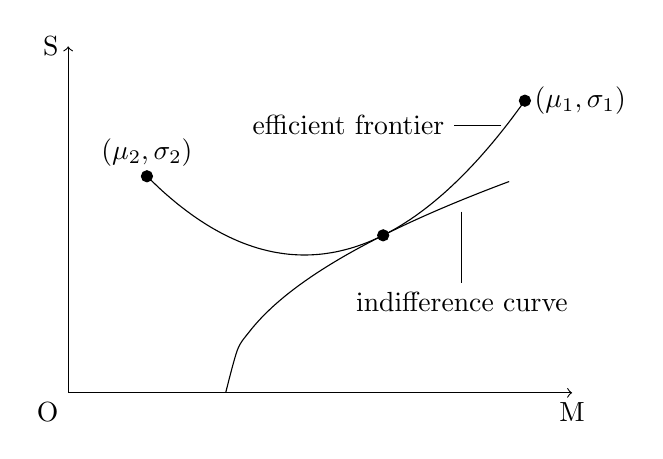
\begin{tikzpicture}[scale=2]
    % 绘制坐标轴
    \draw[->] (0,0) -- (3.2,0) node[below] {M};
    \draw[->] (0,0) -- (0,2.2) node[left] {S};
    \draw[black] (0,0) node[below left] {O};

\draw[domain=1:2.8,smooth,variable=\x, black] plot ({\x},{sqrt(\x-1)}) ;
\draw[domain=0.5:2.9,smooth,variable=\x, black] plot ({\x},{0.5* \x * \x -1.5* \x +2 }) ;

\filldraw [black] (2,1) circle (1pt)   ;
\filldraw [black] (0.5,1.375) circle (1pt)   ;
\draw[black] (0.5,1.375) node[above] {($\mu_2, \sigma_2$)};

\filldraw [black] (2.9,1.855) circle (1pt)   ;
\draw[black] (2.9,1.855) node[right] {($\mu_1, \sigma_1$)};

\draw[black] (2.5,1.15) -- (2.5,0.7) node[below ] {indifference curve};
\draw[black] (2.75,1.7) -- (2.45,1.7) node[left ] {efficient frontier};

\end{tikzpicture}
\caption{Portfolio choice in mean-variance framework} %最终文档中希望显示的图片标题
\label{Fig9.1} %用于文内引用的标签
\end{figure}

Next suppose there is one riskless asset with a sure gross return $\mu_0$, and risky assets are as before. If a fraction $x_0$ of wealth is held in the riskless asset, then
\begin{equation*} 
M = x_0 \mu_0 + x^T \mu = x_0 \mu_0 + (1-x_0) \xi^T  \mu
\end{equation*}
where the vector $\xi$ gives the proportions of the various assets in the risky part of the portfolio. Likewise,
\begin{equation*} 
S^2 = x^T \Sigma x = (1-x_0)^2 \xi^T \Sigma \xi
\end{equation*}
or
\begin{equation*} 
 S=(1-x_0) (\xi^T \Sigma \xi)^{1/2}
\end{equation*}
Therefore the feasible points are found by joining $(\mu_0, 0)$ to each of the points on the frontier previously obtained. In Figure \ref{Fig9.2}, this produces the efficient frontier $ABP_1$ if short sales are not allowed, and the straight-line frontier $ABC$ if they are. In this case the risky assets are only ever held in the proportions represented by the point $B$. Everyone holds a mix of the sure asset and the portfolio $B$, the proportions of this mix depending on the attitude to risk. Thus $B$ becomes a mutual fund.

\begin{figure}[!htb] %H为当前位置,!htb为忽略美学标准,htbp为浮动图形
\centering %图片居中
%\includegraphics[width=0.8\textwidth]{./Fig3.1.png} %插入图片,[]中设置图片大小,{}中是图片文件名
\begin{tikzpicture}[scale=2]
    % 绘制坐标轴
    \draw[->] (0,0) -- (3.2,0) node[below] {M};
    \draw[->] (0,0) -- (0,2.2) node[left] {S};
    \draw[black] (0,0) node[below left] {O};

\draw[domain=0.5:2.9,smooth,variable=\x, black] plot ({\x},{0.5* \x * \x -1.5* \x +2 }) ;

\filldraw [black] (2.2,1.12) circle (1pt) node [below right] {B} ;
 
\draw[black] (0.5,1.375) node[above] {$P_2$};
 
\draw[black] (2.9,1.855) node[above] {$P_1 $};
\draw[-] (0.6,0) -- (3,1.68) node[right] {C};
\draw[black] (0.6,0) node[below ] {A};
\end{tikzpicture}
\caption{Portfolio choice with a riskless asset} %最终文档中希望显示的图片标题
\label{Fig9.2} %用于文内引用的标签
\end{figure}

\section*{Examples}

\subsubsection*{\textit{Example 9.1: Managerial Incentives}}

Eliciting the right amount of effort from subordinates is a problem for capitalist owners and socialist planners alike. Here is a simple example. An owner has to hire a manager to run a project. If the project succeeds, it will produce value $V$. The probability of success depends on the quality of the manager's work. Given high quality, the project will succeed with probability $p$, but low quality will reduce this to $q$. The basic salary needed to attract a manager is $w$. But he has to exert himself  more to achieve high quality, and will do so only if he is paid a premium $e$. Both the owner and the manager are risk-neutral, that is, each maximizes the mathematical expectation of his monetary returns (minus the money-equivalent cost of effort in the case of the manager).

First suppose the owner can observe the quality of the manager's work, and compensate the effort directly. His expected profit from eliciting high-quality work is $pV - (w+e)$, while low-quality operation would get him $qV-w$. The interesting case to consider is one where (a) high quality yields more profit than low quality, that is
\begin{equation} \label{equa9.15}
pV - (w+e) > qV -w \quad \mbox{or} \quad (p-q)V >c
\end{equation}
and (b) the profit with high quality is positive, that is,
\begin{equation} \label{equa9.16}
pV >w+c
\end{equation}

Now suppose the owner cannot observe the quality of effort. If the owner offers the premium $e$ to a manager in return for an unverifiable promise to provide high-quality work, the manager can cheat and deliver low quality instead. This lowers the probability of success of the project, but so long as $1>p>q>0  $, the owner cannot infer the quality of the manager's effort by observing a single success or failure, and therefore has no recourse against the manager's breach of contract.

Therefore the owner must base his payment scheme on the only thing he can observe, namely success or failure. Suppose he pays the manager $x$ if the project succeeds, and $y$ if it fails. Given this scheme, the manager will choose high-quality effort if this gives him greater benefit net of the cost of his effort, that is, if 
\begin{equation*}
px + (1-p)y -e > qx + (1-q)y 
\end{equation*}
If the two sides are equal, the manager is indifferent between high and low-quality effort. It is usual to suppose that so long as it makes no difference to him, he acts like a nice guy and breaks the tie favorably to the owner, that is, chooses high quality. Therefore the inequality is weak rather than strict. It simplifies to 
\begin{equation} \label{equa9.17}
(p-q) (x-y) \geq e
\end{equation}
Secondly, the manager will agree to work for the owner if 
\begin{equation*}
px + (1-p)y \geq w + e
\end{equation*}
or 
\begin{equation} \label{equa9.18}
 y + p(x-y) \geq w+e
\end{equation}
These then are the constraints that give the manager the right incentives.

The owner's expected profit is 
\begin{equation} \label{equa9.19}
\pi = pV - [  px + (1-p)y  ] = pV -y -p(x-y)
\end{equation}
He wants to maximize this subject to the two incentive constraints above. It is obvious that he should make $y$ and $(x-y)$ as small as possible. Then the constraints will hold with equality, and 
\begin{equation*} 
 x-y = e/(p-q) \quad y =w+e - ep/(p-q)
\end{equation*}
or
\begin{equation} \label{equa9.20}
 y = w -e q/(p-q) \quad  x = w +e (1-q)/(p-q)
\end{equation}
These have a simple interpretation: the manager's compensation consists of the basic salary plus a reward for success or minus a penalty for failure.

With these values, the owner's expected profit is
\begin{equation*} 
\pi = pV - w-e
\end{equation*}
the same as when he could observe the manager's effort directly; the inability to observe effort has made no difference.

But there is a difficulty. Nothing guarantees $y \geq 0$. Thus the optimum scheme may involve a fine that the manager pays to the owner if the project fails. In practice such a fine is very difficult to extract. If fines are ruled out, the problem must be solved with an additional constraint $y \geq 0$. The solution is to go as far as possible, namely set $y=0$. Then $x$ must satisfy the remaining two constraints, so 
\begin{equation*}
x \geq (w+e)/p \quad \mbox{and} \quad x \geq e/(p-q)
\end{equation*}
But when the $y$ in the unconstrained solution is negative, $w+e$ is less than $ep/(p-q)$, and the latter is the binding constraint. So $x=e/(p-q)$, and the owner's expected profit is 
\begin{equation*} 
\pi = pV - ep/(p-q)
\end{equation*}
By the conditions (\ref{equa9.15}-\ref{equa9.16}) assumed at the outset, this is less than $pV - w-e$, but still positive. Thus the need to pay output-based incentives means a smaller expected profit, but not by so much as to make the whole enterprise unprofitable.

This example is just the beginning of a large body of recent research on the design of incentive contracts. The problem considered here is similar to that of moral hazard in insurance, where the company could not observe the risk-reducing care on the part of the policyholder. We designed the best contract for a single project. In an ongoing relationship of this kind, the average of the manager's successes over time provides statistical information about his effort, enabling a better contract that generates higher expected profit. Similarly, if the planner has several similar managers who face some common risk, then observation of their relative performance can provide information about their relative efforts. Finally, in the example there was a liquidity constraint - the manager could not be fined - but no risk-aversion. Allowing the manager to be risk-averse brings additional issues of the efficient allocation of risk between the planner and the manager. Some references to the burgeoning literature on such matters are provided at the end of the chapter.

The next example concerns a different problem of information. The planner may not know the innate quality of the manager. This, too, has a parallel in insurance, where the policyholder has better information about his own risk-class than does the company. This gives rise to `adverse selection'; an insurance policy is especially attractive to those who know their own risk to be higher than the odds implicit in the terms of the policy, and who are therefore undesirable customers from the point of view of the company. It wants to design a contract that will handle this problem. For variety, I shall construct the example in a different context.

\subsubsection*{\textit{Example 9.2: Cost-Plus Contracts}}

Government expenditures for defense, health, and yes, even education are often made on a cost-plus basis. That is, the government reimburses the supplier's cost plus a normal profit. The government's purchasing agency usually does not know the true cost of production of these goods or services. If a supplier who can produce the good at low cost pretends to have a higher cost, he gets a higher reimbursement, which he can enjoy by paying high salaries to himself and other workers, spending lavishly on offices and such facilities etc. If the government wishes to avoid the excessive payment, it must devise a scheme that eliminates the temptation to misstate cost. Here is a very simple example.

Suppose the true average cost of production can take just one of two values, $c_1$ and $c_2$, with $c_1 < c_2$. Each figure already includes normal profit. The problem is that the higher figure may be real or pretense; the government cannot tell the difference. In other words, the supplier can be either of two types, low cost or high cost, and the purchasing agency cannot tell whether if faces a genuinely high-cost supplier, or a type-$c_1$ who is pretending to be a type-$c_2$ and planning to enjoy the extra payment.

The government can decide how many units it will buy, and how much it will pay, depending on the cost declared by the supplier. Suppose it announces that if the supplier claims to have the average cost $c_i$, for $i=1$ or 2, it will buy $q_i$ units, and pay a total sum of $R_i$ for them.

What are the constraints on these choices? First, for each of the two cost figures, if that happens to be genuine, the supplier should be willing to participate. That is, his cost should be covered:
\begin{equation} \label{equa9.21}
R_i \geq c_i q_i \quad \mbox{for} \ i=1,2
\end{equation}
Secondly, it should be optimal for the supplier to reveal his true cost. These are called incentive compatibility constraints. If the supplier's true average cost is $c_1$, he should not wish to pretend it is $c_2$, and the other way round. Economic intuition suggests that only the first of these will be binding (a truly high-cost firm will not pretend to be low-cost), but a proper theoretical treatment should prove that, and not assume it at the outset. Now if a firm with cost $c_1$ pretends to have cost $c_2$, it sells $q_2$ units instead of $q_1$, and has revenue $R_2$ instead of $R_1$, but its actual cost in its profit calculation stays at $c_1$. Therefore the constraint for a firm with cost $c_1$ to report it truthfully is 
\begin{equation}\label{equa9.22}
R_1 - c_1 q_1 \geq R_2 - c_1 q_2
\end{equation}
Similarly for a firm with true cost $c_2$, the constraint is 
\begin{equation} \label{equa9.23}
R_2 - c_2 q_2 \geq R_1 - c_2 q_1
\end{equation}

Suppose the government gets benefit $B(q)$ from quantity $q$, where $B$ is an increasing and strictly concave function. Suppose its estimate of the probability of the true cost being $c_1$ is $\theta_1$, and that of $c_2$ is $\theta_2 = 1- \theta_1$. Then its expected benefit net of the payments to the supplier is 
\begin{equation} \label{equa9.24}
\theta_1 [B(q_1) - R_1] + \theta_2 [B(q_2) - R_2]
\end{equation}
The optimum scheme will maximize this subject to the participation and incentive compatibility constraints (\ref{equa9.21},\ref{equa9.22},\ref{equa9.23}). For the moment I shall ignore non-negativity constraints on the $q_i$ and $R_i$.

Form the Lagrangian
\begin{equation*}
\begin{array}{rl}
L =& \theta_1[B(q_1) - R_1] + \theta_2 [B(q_2) - R_2] \\
   & + \mu_1 [R_1 -c_1 q_1] + \mu_2 [R_2 - c_2 q_2] \\
   & + \lambda_1 [R_1 - R_2 - c_1 q_1 + c_1 q_2] +  \lambda_2 [R_2 - R_1 - c_2 q_2 + c_2 q_1]
\end{array}
\end{equation*}

Most of the economically interesting results can be found without solving the whole problem. First we add the incentive compatibility constraints together and simplify to write
\begin{equation} \label{equa9.25}
 (c_2 - c_1) (q_1 - q_2) \geq 0
\end{equation}
so if the supplier declares lower cost, he will sell at least as much, and typically more. This is a part of the incentive for the low-cost-type firm to respond truthfully. Indeed the solution may have $q_2 =0$ and $q_1 >0$. That will effectively eliminate the incentive to pretend to have high cost. But this carries a risk: if the supplier turns out to have genuinely high cost, the government, having committed itself to the scheme, will be unable to purchase from him even though such a transaction might be \textit{ex post} desirable. Therefore such a solution will arise only if either this risk or its consequences are sufficiently small, that is, if $\theta_2$ is small, or $B^\prime(0)$ is finite and small. I shall leave the details to the reader, and assume henceforth that $q_2$ and $q_1$ are both positive.

Now consider the participation constraints (\ref{equa9.21}). The aim is to prove that both cannot be slack. Begin by noting that if a type-2 firm makes positive profit, so does a type-1 firm. To see this, suppose $R_2 - c_2 q_2 > 0$, then from type-1's incentive compatibility constraint (\ref{equa9.22}) we have
\begin{equation*}
R_1 - c_1 q_1 > (c_2 - c_1) q_2 > 0
\end{equation*}
Next note the first-order conditions for $R_1$ and $R_2$:
\begin{equation*}
-\theta_1 + \lambda_1 - \lambda_2 + \mu_1 =0
\end{equation*}
\begin{equation*}
-\theta_2 - \lambda_1 + \lambda_2 + \mu_2 =0
\end{equation*}
In firms of both types make positive profits, both participation constraints are slack, and complementary slackness implies $\mu_1 = 0 = \mu_2$. Then
\begin{equation*}
\theta_1 = \lambda_1 - \lambda_2 = - \theta_2
\end{equation*}
but both $\theta_1$ and $\theta_2$ are positive, so this is impossible.

Therefore the optimum scheme must have
\begin{equation} \label{equa9.26}
R_2 - c_2 q_2 =0  \quad R_1 - c_1 q_1 > 0
\end{equation}
The positive pure profit is another part of the incentive a type-1 firm has for revealing its low cost truthfully. Its average revenue $R_1 /q_1$ exceeds its average cost $c_1$, but by type-2's incentive compatibility constraint, it cannot exceed $c_2$.

Of course the government will make $R_1$ as small as possible while meeting type-1's incentive compatibility constraint (\ref{equa9.22}). Substituting for $R_2$ in it, we have
\begin{equation} \label{equa9.27}
R_1 = c_1 q_1 + (c_2 - c_1) q_2
\end{equation}
With this, it is easy to verify that (\ref{equa9.23}) is automatically satisfied, and it is a strict inequality so long as $q_1 > q_2$ which is true at the optimum. Thus we have proved the intuitive suggestion that the truly high-cost firm will not want to deflate its cost, but the truly low-cost firm will be on the verge of wanting to inflate its cost.

Now the government's objective function can be rewritten as 
\begin{equation*}
\theta_1  [B(q_1) - c_1 q_1 - (c_2 - c_1)q_2] + \theta_2[B(q_2) - c_2 q_2]
\end{equation*}
The first-order conditions with respect to $q_1$ and $q_2$ are
\begin{equation} \label{equa9.28}
B^\prime(q_1) = c_1
\end{equation}
and
\begin{equation} \label{equa9.29}
B^\prime(q_2) = c_2 + (\theta_1/\theta_2)(c_2 - c_1)
\end{equation}

These have a role in the incentive scheme, too. Of the two, (\ref{equa9.28}) is straightforward. If the supplier declares himself to be low-cost, the government buys from him a quantity that makes the marginal benefit equal to the marginal (equals average) cost. But (\ref{equa9.29}) is more complicated. If the supplier declares himself to be high-cost, that in itself would be a reason for buying less; the equality of marginal benefit and cost would imply $B^\prime(q_2)=c_2$ and therefore $q_2 < q_1$. In fact the right-hand side of (\ref{equa9.29}) is greater than $c_2$, so the government buys even less from a high-cost supplier. This again makes it less tempting for the low-cost supplier to inflate cost. The policy does mean giving up a net marginal social gain when the supplier is really of type 2, but it is desirable to incur some such cost to achieve the offsetting gain on the incentive side. Another way of expressing the idea is to note that the possibility of the cost being higher offers a temptation for the low-cost firm to pretend a high cost; this is like an external diseconomy caused by a high-cost firm. The right-hand side of (\ref{equa9.29}) adds the shadow cost of this externality to $c_2$ to get the true social cost of a type-2 firm. Then the amount $q_2$ bought from it equates the marginal benefit with this true social cost.

\subsubsection*{\textit{Example 9.3: The Mean-Variance Frontier}}

Here I examine the convexity of the transformation frontier in portfolio selection with $n$ assets. This fills out the technical details omitted from the text, and incidentally provides a nice illustration of the use of convexity and maximum-value functions. The argument proceeds using two intermediate results or lemmas.

\textit{Lemma 1:} $\phi(x) = (x^T \Sigma x)^{\frac{1}{2}}$ is a convex function of $x$.

\textit{Proof:} Let $\phi^2 = x^T \Sigma x$, then differentiating,
\begin{equation*}
 2 \phi \phi_x = 2 \Sigma x
\end{equation*}
and
\begin{equation*}
  \phi \phi_{xx} + \phi_x \phi_x^T =  \Sigma 
\end{equation*}
Therefore
\begin{equation*}
 \phi \phi_{xx} =  \Sigma x - \dfrac{\Sigma x x^T \Sigma}{\phi^2}
\end{equation*}

We show that the matrix $\phi_{xx}$ is positive semi-definite. For any vector $z$,
\begin{equation*}
\begin{array}{rl}
 \phi z^T \phi_{xx} z &= z^T \Sigma z - z^T \Sigma x x^T \Sigma z / \phi^2 \\
                      &= z^T \Sigma z - (z^T \Sigma x)^2 /(x^T \Sigma x)
\end{array}
\end{equation*}
This expression is non-negative by the Cauchy-Schwartz inequality.

\textit{Lemma 2:} If $\phi(x)$ is convex, and
\begin{equation*}
S = \min \{ \phi(x) \ | \ \mu^T x = M, e^T x =1   \}
\end{equation*}
then $S$ is a convex function of $M$.

\textit{Proof:} Let $M_1$, $M_2$ be any two values of $M$, and let $x^1$, $x^2$ the respective minimizers. Then for any $\theta \in [0,1]$,
\begin{equation*}
\mu^T [\theta x^1 + (1-\theta)x^2] = \theta M_1 + (1-\theta) M_2
\end{equation*}
\begin{equation*}
e^T  [\theta x^1 + (1-\theta)x^2] = 1
\end{equation*}
So the average portfolio is feasible. Therefore
\begin{equation*}
\begin{array}{rl}
 S[\theta M_1 + (1-\theta)M_2] &\leq \phi [\theta x^1 + (1-\theta)x^2] \\
                      &\leq  \theta \phi(x^1) + (1-\theta)\phi(x^2) \\
                       &= \theta S(M_1) + (1-\theta)S(M_2)
\end{array}
\end{equation*}

This proves the desired convexity. Now I indicate how to obtain the explicit solution for the frontier $S(M)$. It is easier to minimize $S^2$. Let $\alpha$, $\beta$ denote the multipliers on the respective constraints. The first-order condition is 
\begin{equation*}
 \Sigma x = \alpha \mu + \beta e
\end{equation*}
Solving for $x$ and substituting in the constraints,
\begin{equation*}
\alpha (\mu^\prime \Sigma^{-1} \mu) + \beta (e^\prime \Sigma^{-1} \mu) = M
\end{equation*}
\begin{equation*}
\alpha (\mu^\prime \Sigma^{-1} e) + \beta (e^\prime \Sigma^{-1} e) = 1
\end{equation*}
These two equations can be solved for $\alpha$ and $\beta$, which in turn gives expressions for the optimum portfolio $x$ and the minimized $S$ in terms of $M$.

\section*{Exercises}

\subsubsection*{\textit{Exercise 9.1: Taxation of Risky Income}}

Suppose that in the model of one safe and one risky asset in the text, we introduce taxation of interest income on the risky asset (with deduction allowed for losses) at the rate $\tau$, where $0<\tau<1$. Thus the final random wealth is 
\begin{equation*}
W = W_0 + (1-\tau)xr
\end{equation*}
Show that the first-order condition for an interior optimum $x$ is
\begin{equation*}
\int_{\underline{r}}^{\overline{r}}  r U^\prime [W_0 +(1-\tau)xr ] f(r) dr = 0
\end{equation*}
Deduce that if $\tau$ changes, the optimum $x$ changes keeping $(1-\tau)x$ constant. Therefore if the tax rate on risky income increases, so does the amount of wealth held in the risky asset. Suggest an economic intuition for this seemingly paradoxical result.

\subsubsection*{\textit{Exercise 9.2: Saving with Uncertainty}}

A consumer lives for two periods. Income in period 1 is sure and equal to $Y_1$. The income $Y_2$ in period 2 can be random. If he saves $S$ from his period-1 income, he gets total return (principal plus interest) of $rS$ in period 2, where $\tau$ can be random. His objective is to maximize the expected present value of the utilities of consumption in the two periods:
\begin{equation*}
U(Y_1 - S) + \delta E[U(Y_2 + rS)]
\end{equation*}
where $U^\prime >0$ and $U^{\prime \prime} <0$. Write down the first- and second-order conditions. Show that as $Y_1$ increases, $S$ also increases but at a smaller rate, that is, the marginal propensity to save lies between 0 and 1.

Next suppose that $Y_2$ is sure but $r$ is random, and examine the effect of an increase in $Y_2$. Finally, suppose $r$ is sure but $Y_2$ random, and examine the effect of an increase in $r$.



